\section{Method}
\label{method}

We consider an utterance in a source language represented as
a monophonic waveform $X \in\mathbb{R}^{f_s \cdot d}$, sampled at a frame rate $f_s = 24\,\mathrm{kHz}$, of duration $d$.
Similarly, its translation is given in a target language,
denoted $Y \in \mathbb{R}^{f_s \cdot d}$. We assume $X$ is padded to ensure both have the same duration. Our objective is to model $\proba{Y | X}$. Contrary to \citet{hibiki}, we do not constrain the modeling of $Y$ knowing $X$ to be entirely causal in our training data. Thanks to the diversity of causality and latency arrangements in the dataset, it is still possible to learn a base translation model. Its behavior is then adjusted by an online reinforcement learning strategy that rewards correct and simultaneous translations.

\subsection{Modeling}
\label{sec:modeling}

We build on the framework introduced by \citet{moshi} for the joint modeling of
multiple sequences of tokens and used by \citet{hibiki} to perform simultaneous S2TT and S2ST with high fidelity.


\subsubsection{Neural audio codec}
\label{sec:neural_audio_codec}

We use the pre-trained causal and streaming Mimi codec~\citep{moshi} to encode $X$ and $Y$ into low framerate sequences of discrete tokens.
Mimi consists of an encoder and decoder from and to the waveform domain, and of an information bottleneck using Residual Vector Quantization (RVQ)~\cite{soundstream}.

For language modeling, we are interested in the discrete
indices of codebook entries which Mimi latents are projected to. We denote those $(A_{t, q}) \in \{1, \ldots, N_a\}^{f_r \cdot d \times Q}$ where $f_r = 12.5 \,\text{Hz}$ is the codec framerate, $Q$ is the number of audio residual quantization levels varying up to 32 and $N_a$ the codebooks size. Following~\citet{zhang2024speechtokenizer,moshi}, the output
of the first quantization level is trained to replicate semantic information
obtained from a WavLM self-supervised audio model~\citep{wavlm}. We refer to $A_{t, 1}$ as \emph{semantic} tokens, and $A_{t, q \geq 2}$ as \emph{acoustic} tokens with the latter arranged in a coarse to fine manner. We keep only $Q=16$ acoustic levels which is sufficient to ensure high quality speech.

\begin{figure}[t]
    \centering
    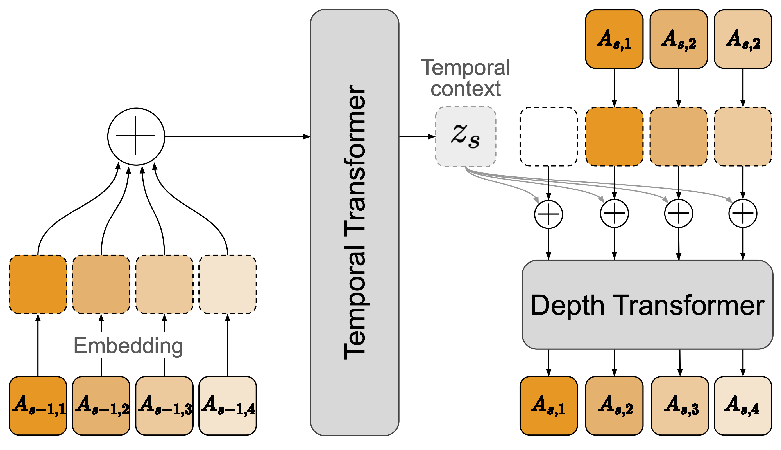
\includegraphics[width=0.8\columnwidth]{figures/hibikzero_rq_transformer.pdf}
    \caption{\textbf{Architecture of the RQ-Transformer.} Figure adapted from ~\citet{moshi}.}
    \label{fig:rq-transformer}
\end{figure}

\begin{figure}[t]
    \centering
    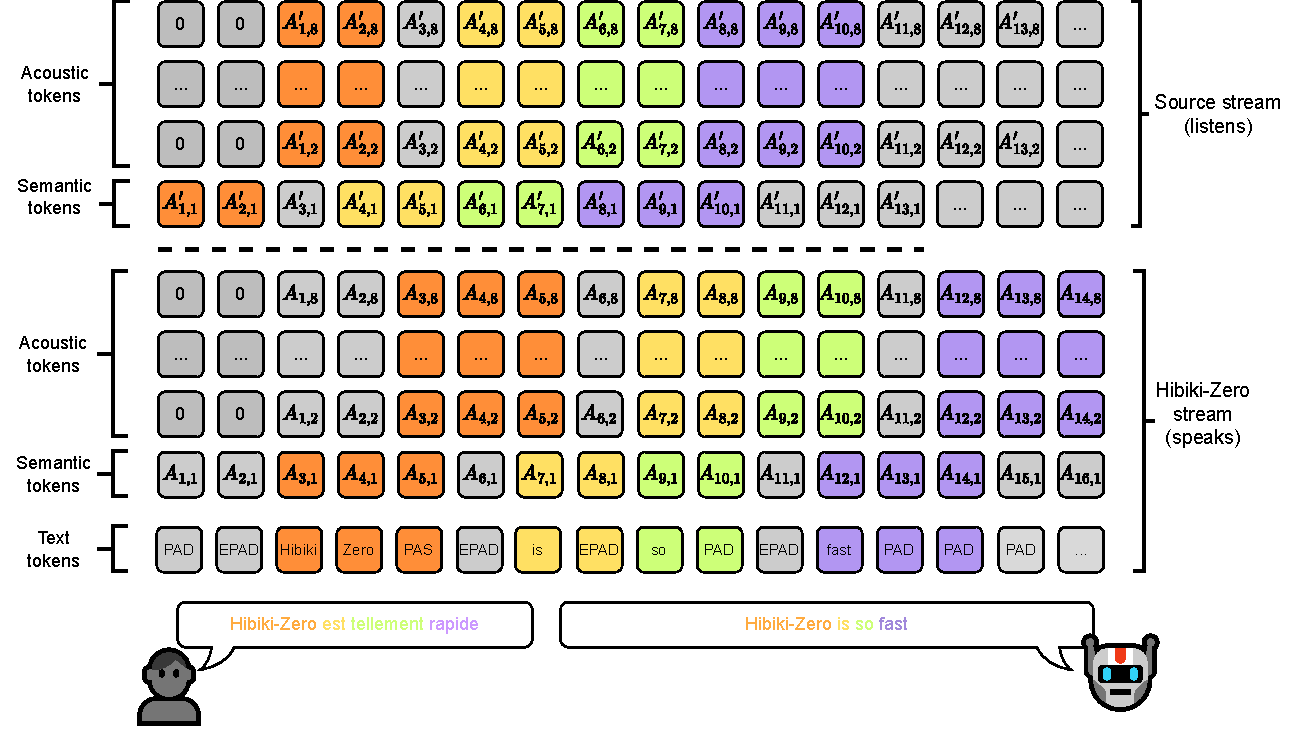
\includegraphics[width=\columnwidth]{figures/text_delays_tokens_hibikizero.pdf}
    \caption{\textbf{Joint sequence modeling.} From the source stream, \ours{} predicts its Inner Monologue text stream, semantic and acoustic tokens. Figure adapted from ~\citet{hibiki}.}
    \label{fig:joint-modeling}
\end{figure}

\subsubsection{Joint modeling of discrete audio tokens}
\label{sec:joint_modeling}

Following \citet{uniaudio,hibiki}, we leverage a RQ-Transformer~\citep{rq-transformer} as shown in Figure~\ref{fig:rq-transformer} to model $(A_{t, q})$ both over the time $t$ and quantizer $q$ axes as audio streams cannot be reasonably merged into a single discrete sequence.
It consists in a large \emph{Temporal} Transformer~\citep{attentionvaswani} of latent dimension $D$, operating at the same framerate $f_r$ as the codec, and being fed all the tokens generated so far, e.g.
for all $t \leq f_r \cdot d$, 
 \begin{equation}
 \label{eq:temp_transformer}
Z_t = \mathrm{Temp}(A_0, \ldots, A_{t - 1}) \in \mathbb{R}^{D}.
\end{equation}
$A_0$ is defined as a deterministic token indicating the start of the generation.
Then, a smaller scale \emph{Depth} Transformer models auto-regressively
the tokens $A_{t, 1}, \ldots, A_{t, Q}$ over the quantizer axis, e.g. for all $t \leq f_r \cdot d$ and $q \leq Q$,
\begin{equation}
\label{eq:dep_transformer}
    l_{t, q} = \mathrm{Dep}(Z_t, A_{t, 0}, \ldots, A_{t, q - 1}) \in \mathbb{R}^{N_a},
\end{equation}
with $A_{t, 0}$ also a special token, and with the goal of having,
\begin{equation*}
    \softmax(l_{t, q}) \approx \proba{A_{t, q} | A_{0}, \ldots, A_{t-1}, A_{t, 0}, \ldots A_{t, q - 1}}
\end{equation*}

Following \citep{musicgen,moshi}, we introduce an acoustic delay shifting acoustic tokens of 2 time steps in the future compared to the semantic stream. The streams are realigned before decoding the audio with the codec. As this delay is always applied, we don't introduce new notations for readability and refer to $(A_{t,q})$ directly.

\subsubsection{Translation as multistream modeling}
\label{sec:multistream_modeling}

Using the RQ-Transformer given by Eq.~\eqref{eq:temp_transformer} and \eqref{eq:dep_transformer} to jointly model multiple discrete streams of tokens, we can perform the task of joint simultaneous S2TT and S2ST as illustrated in Figure~\ref{fig:joint-modeling}.
Following~\cite{moshi}, we use an \textit{Inner Monologue} by introducing a stream of padded text tokens $(W_t) \in \{1, \ldots, N_W\}^{f_r \cdot d}$ whose content is the aligned text transcription of the audio modeled in $A^Y$. This text stream is concatenated with the audio tokens $A^Y$ from the source interpretation along the $q$-axis such that it comes before the semantic level.
Then, we concatenate the target tokens $A^Y$ and source tokens $A^X$ along the $q$-axis.
At inference time, predictions of tokens $A^X$ are skipped and actual tokens of the input audio are used instead.

\subsubsection{Architectural details}
\label{sec:arch_details}

At time-step $t$, tokens from the previous step, e.g. $A^X_{t-1}$,
$A^Y_{t-1}$, and $W_{t-1}$, are fed into dedicated embedding tables and contributions are summed with a BOS token used for the first time step $t = 1$.
The RQ-Transformer uses standard Transformer layers~\citep{attentionvaswani}, with gated SiLU activation~\citep{shazeer2020glu,hendrycks2016gaussian}.
A linear layer maps output $Z_t$ of the \emph{Temporal} Transformer to logits for the text token $W_t$.
The \emph{Depth} Transformer then operates for $Q$ steps to estimate the logits for the output stream and for $Q$ additional steps for the input stream.
Each depth step $q$ takes as input $Z_t$ summed with a learned embedding of the previous audio token $A_{t, q - 1}$, or $W_t$ for $q = 1$.
We provide architectural hyper-parameters in Section~\ref{sec:arch_hyper_params}.


%%% SECTION %%%
\subsection{Coarse alignment of speech translation data}
\label{sec:synth_st_data}

We have assumed training pairs $(X, Y)$ to not be entirely causal at the interpretation level. We now detail the specific method used to build such coarse translation alignments.

\subsubsection{Sentence-level alignment}
\label{sec:sent_level_align}

We start from an unaligned speech translation pair $(X, Y)$ which only verifies a sentence mapping constraint meaning that both $X$ and $Y$ contain the same number of sentences and such that the $i^{th}$ sentence in $Y$ is a translation of the $i^{th}$ sentence in $X$. Inspired by \citet{hibiki}, we rely on the insertion of artificial silence in $Y$ to delay its content with respect to $X$.  For each sentence of index $i$, we introduce silence in $Y$ to shift its $i^{th}$ sentence by an amount $\delta_i$ after the start of the $i^{th}$ sentence in $X$ where $\delta_i \sim \mathcal{U}(0,\delta \times d_{i})$ is sampled independently for each sentence, $d_{i}$ is the duration of the $i^{th}$ sentence in $X$ and $\delta \in [0,1]$ is an hyperparameter. Then, using punctuation characters such as commas or colons in a precomputed transcript of $Y$, we insert silences whose durations follow $\mathcal{U}(0,\mu)$ at the corresponding instants in $Y$ with $\mu$ being a hyperparameter.

\subsubsection{Natural pauses TTS}
\label{sec:nat_pauses_tts}

Using the method described in Section \ref{sec:sent_level_align}, we might break the natural flow of speech by inserting silence on punctuations which is also subject to imprecisions of the transcript timestamps. Following \citet{dsm}, we train a TTS with synced audio and text streams as output, providing a control on the emission timestamp of each word to synthesize. Moreover, we train the TTS to perform voice transfer from a short audio conditioning of maximum 10 seconds. We can then generate an audio $Y^+$ using the original transcript of $Y$ and naturally insert the pauses described in \ref{sec:sent_level_align} while conditioned on the speaker from $X$. This results in new training pairs ($X$, $Y^+$) where targets contain smoother transitions between speech and silences than $Y$.


%%% SECTION %%%
\subsection{Translation policy reinforcement}
\label{sec:rl_method}
Assuming that we dispose of a simultaneous translation model as presented in Section~\ref{sec:modeling}, we now introduce a reinforcement learning procedure using process rewards based on BLEU scores to improve the translation policy of the model as illustrated in Figure~\ref{fig:rewards_pattern}. We adapt GRPO from \citet{grpo} to be our RL algorithm. We denote by $\pi_{\theta}$ the translation model to optimize and $\pi_{\theta_{\mathrm{old}}}$ an older version of it acting as a regularizer. Given an input speech utterance $X$ with a known sentence-level text translation $y$, we use $\pi_{\theta_{\mathrm{old}}}$ to generate $G$ different speech translations $(Y_i)_{1 \le i \le G}$, each of duration $T \times f_r$ seconds where $f_r$ is the model frame rate and $T$ a fixed number of frames.

\subsubsection{Process rewards}
\label{sec:process_rewards}

\looseness=-1
Let $n$ be the number of sentences in $X$ and $(t_i)_{0 \le i \le n}$ the frame indexes such that the sentence of index $i$ in $X$ starts at frame $t_i$ and ends at frame $t_{i+1}$. We introduce $S(t)$ as the sentence index at frame $t \ge t_0$ in $X$ i.e. $S(t)=i$ for $t_i \le t \le t_{i+1}$ and $S(t)=n-1$ for $t > t_n$. For a frame index $t \le T$, we denote $y_t$ as the text concatenation of translated input sentences until the one of index $S(t)$ included. Given a generation $i$, we define $\hat{y}^{(i)}_{t}$ as the partial text transcript until frame $t$ given by the model's output text stream. We now introduce the hyperparameter $\alpha \in [0,1]$ and define the process reward for generation $i$ at frame $t$ as:
\begin{equation}
\label{eq:process_reward}
    r^{(i)}_{t} = (1 - \alpha) \mathrm{BLEU} \big( \hat{y}^{(i)}_{t}, y_{t} \big) + \alpha \mathrm{BLEU} \big( \hat{y}^{(i)}_{T}, y_{T} \big)
\end{equation}

\subsubsection{Optimization objective}
\label{sec:optim_objective}
Using the modeling of $X$ and $(Y_i)_{1 \le i \le G}$ as tokens $A^X$ and $A^{Y_{1}}$, ..., $A^{Y_{G}}$, we define the probability ratios between $\pi_{\theta}$ and $\pi_{\theta_{\mathrm{old}}}$ for each output $i$, codebook index $q \le Q$ and frame index $t \le T$ as:
\begin{equation}
\label{eq:log_prob}
    p^{(i)}_{q,t} = \frac{\pi_{\theta} \Big( A^{Y_{i}}_{q,t}|A^X_{\le t},A^{Y_{i}}_{q,<t} \Big) }{\pi_{\theta_{\mathrm{old}}} \Big( A^{Y_{i}}_{q,t}|A^X_{\le t},A^{Y_{i}}_{q,<t} \Big) }
\end{equation}

Given a set of frame indexes $t'_1 < t'_2 < ...< t'_s$, we compute process rewards as defined in Section~\ref{sec:process_rewards} for each output, namely $r^{(i)}_{t'_{j}}$ for $i \le G$ and $j \le s$. We then normalize rewards per frame index across group elements:
\begin{equation}
\label{eq:norm_reward}
\bar{r}^{(i)}_{t'_{j}} = \frac{r^{(i)}_{t'_{j}} - \underset{k \le G}{\mathrm{mean}} \Big[ r^{(k)}_{t'_{j}} \Big]}{\underset{k \le G}{\mathrm{std}} \Big[ r^{(k)}_{t'_{j}} \Big]}
\end{equation}

In practice, early experiments showed that using a regular frame indexes pattern along the input speech content performed better. Thus we introduce $n_w \in \mathbb{N}^*$ and use the end timestamp of every $n_w$ words in the input to set $(t'_j)_{j \le s}$.

Then, we introduce the advantage of an output at step $t$ as the sum of normalized rewards from the following steps:
\begin{equation}
\label{eq:advantage}
R^{(i)}_t = \sum\limits_{t'_j > t} \bar{r}^{(i)}_{t'_{j}}
\end{equation}

We compute the per-codebook objectives $L^{(i)}_{q}$ using the standard clipping function between $1 - \epsilon$ and $1 + \epsilon$ as:
\begin{equation}
\label{eq:intermediate_objective}
L^{(i)}_{q} = \sum\limits_{t=1}^{T} \min \Big( p^{(i)}_{q,t} R^{(i)}_t, \mathrm{clip}_{\epsilon} \big( p^{(i)}_{q,t} \big) R^{(i)}_t \Big)
\end{equation}

In the end, we seek to maximize the following objective with fixed weights $c_q$ for each depth $q \le Q$:
\begin{equation}
\label{eq:grpo_objective}
\E_{\substack{
X \sim \mathcal{D} \\
Y_i \sim \pi_{\theta_{\mathrm{old}}}(X)
}}
\left[
\frac{1}{G} \sum_{\substack{q \le Q \\ i \le G}} c_q \, L^{(i)}_{q}
\right]
\end{equation}

where $\mathcal{D}$ denotes our input speech distribution and $\pi_{\theta_{\mathrm{old}}}$ is a fixed version of the translation model that is replaced by $\pi_{\theta}$ every fixed number of updates $\tau$.

\begin{figure}[t]
    \centering
    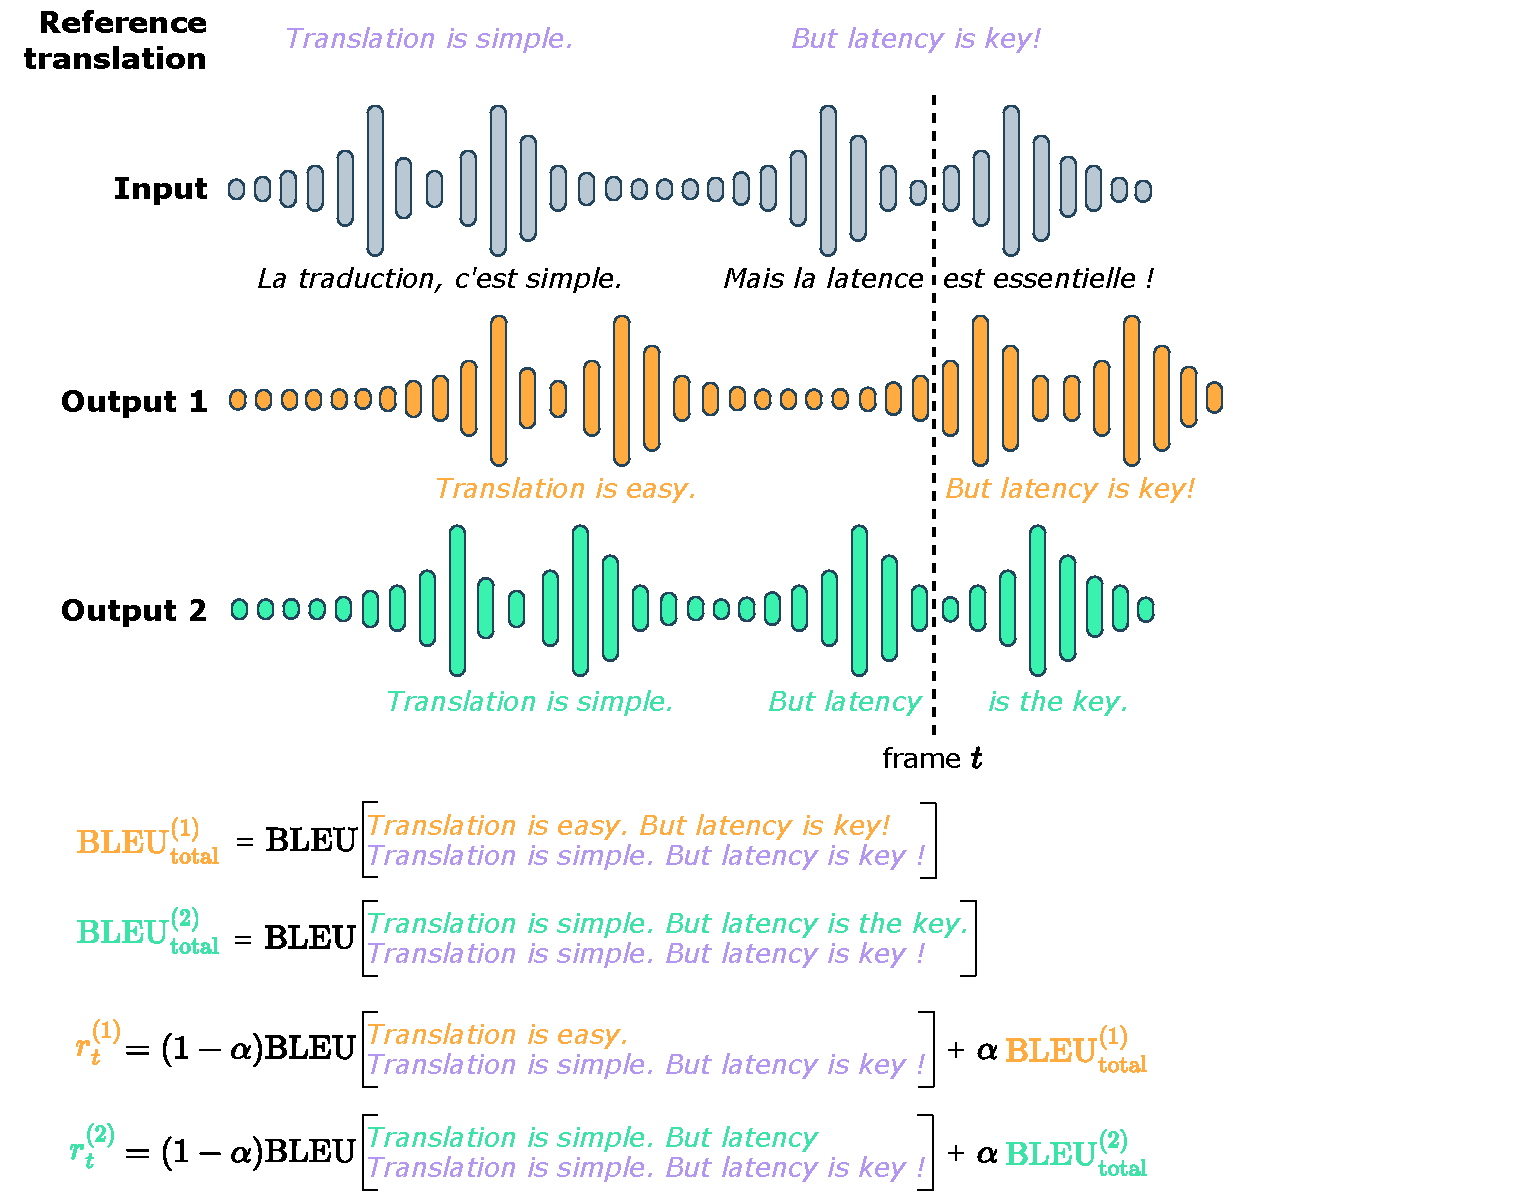
\includegraphics[width=\columnwidth, trim={0 0.03cm 5cm 0}, clip]{figures/rewards_pattern.pdf}
    \caption{\textbf{Process rewards method based on BLEU score.} We introduce intermediate BLEU score computed on the text output of the model before a given frame $t$ and using the ground-truth translation of the corresponding input sentences processed so far. We combine it with the total output BLEU score using $\alpha \in [0,1]$.}
    \label{fig:rewards_pattern}
\end{figure}